\section{Introduction} \label{sec:intro}
Early on in the project, engineering diagrams were produced that describe in great detail the layout of the camera as a whole and of the camera focal plane specifically. See \citeds{LCA-13381} for the latest iteration on these diagrams. The coordinate system was chosen such that a single consistent coordinate system could be applied to the camera, focal plane, rafts, and sensors.

Following the engineering coordinate system all the way down to the sensor level shows that the x-axis happens to align with the parallel transfer direction of the individual segments.

Note that the engineering coordinate system is also used to inform how the various components in the focal plane are named. The naming convention is to index (x, y) from 0 along the positive direction of both axes in engineering coordinates. This leads to names like "R:2,0"\footnote{This specific naming convention is that adopted by the DM subsystem, but is based on the indexing scheme from the camera engineering diagrams} for the raft in the third column of the first row. Similar names apply to sensors within rafts and segments within sensors. This document does not suggest changing the names of the various components, merely that they be displayed in different coordinate systems depending upon context.

\section{Data Visualization}
People conducting data visualization at the sensor level in astronomy are very used to seeing pixel data presented such that the serial register is in a horizontal orientation with the parallel transfer direction oriented vertically. This is primarily because that is the most natural orientation if the serial register is thought of as being clocked out from left to right with parallel transfer thought of as being down. Since bleeding due to saturation is more prominent along the parallel transfer direction, bleed trails are typically shown in the vertical direction.

Because of the long history of astronomers looking at images in the orientation where the serial register is along the x-axis and the parallel transfer direction is along the y-axis, it is highly desirable to maintain the same orientation when view larger chunks of data. That is, maintain this orientation whether visualizing sensors, rafts, or the full focal plane for self consistency. Fortunately, in the design of the LSST camera, the sensors all have the same orientation except for two of the wave front sensors. This makes choosing a coordinate system for data visualization relatively trivial.

Data from DECam, Hyper Suprime-Cam, MegaCam, and others have been successfully processed through LSST code using this convention.

\section{Coordinate Systems}
Since the coordinate system for the engineering diagrams is already decided, the only question is how to map that coordinate system to one where the vertical axis is mapped to the horizontal axis and vice versa. There are two obvious ways to do that:

\begin{itemize}
\item Rotation: A rotation of 90 degrees maps +y -> -x and +x -> +y.
\item Transpose: A transpose maps +y -> +x and +x -> +y.
\end{itemize}

For this situation, the transpose is a much better option because:

\begin{enumerate}
\item It is significantly easier to mentally visualize transposition than rotation.
\item The resulting sky orientation follows the convention preferred by astronomers: +E 90 degrees counterclockwise from +N.  See Figure 1 of data plotted in data visualization coordinates with the celestial coordinate grid overplotted.
\end{enumerate}

\begin{center}
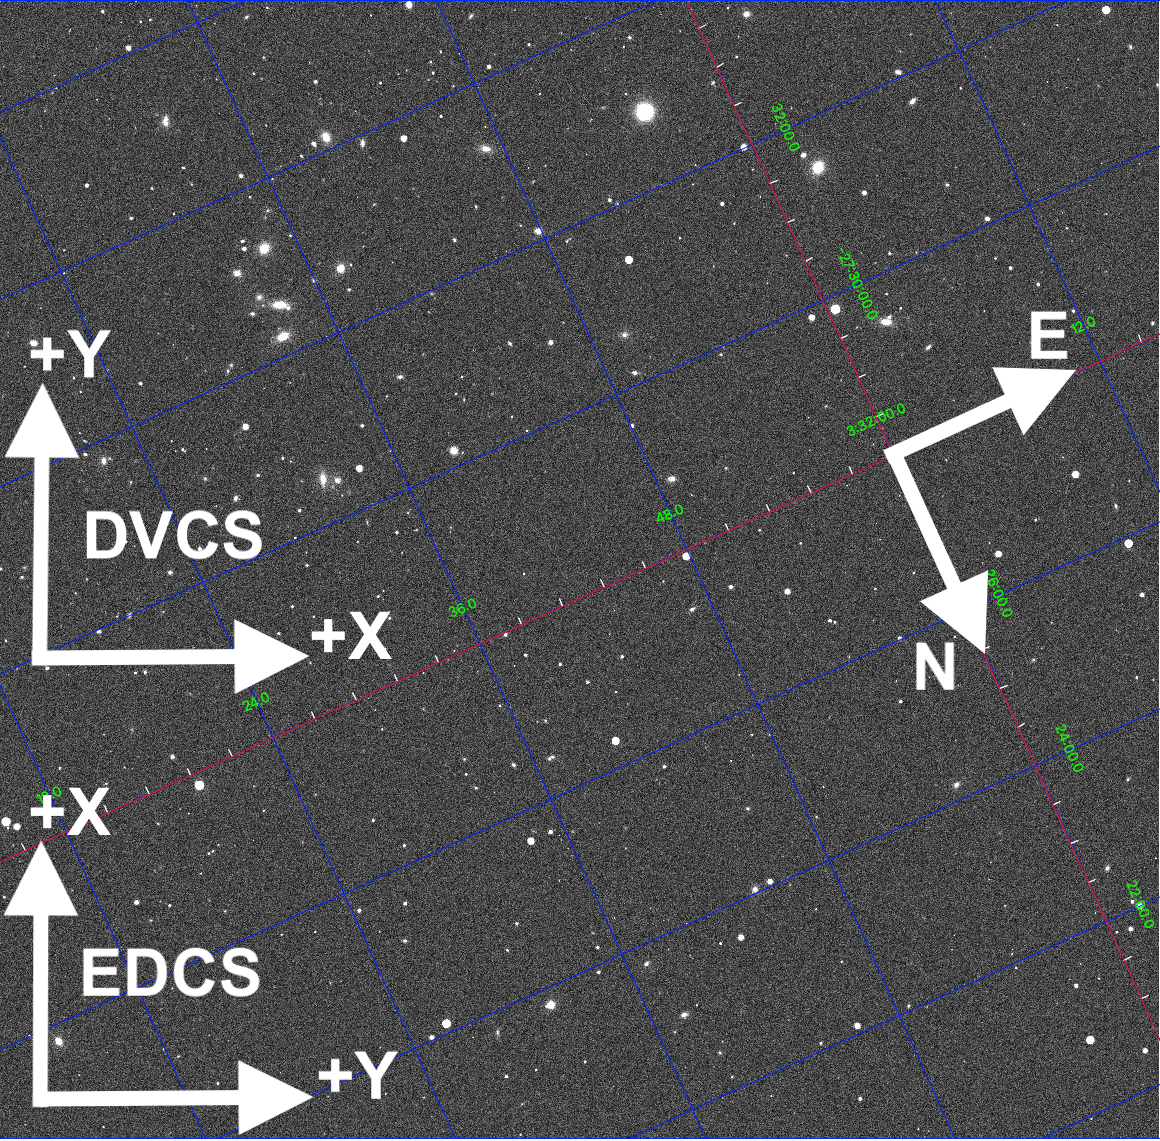
\includegraphics[width=0.75\textwidth]{figures/ds9_coords_with_arrows.png}
\captionof{figure}{This image is in the data visualization coordinate system (DVCS).  The engineering diagram coordinate system (EDCS) is shown in the lower left of the image.  Notice that in these coordinates, east is 90 degrees from north in the counter clockwise direction.}
\end{center}

To be clear, the convention of transposing the engineering diagram coordinate system means that, in the data visualization coordinate system, the pixel grids must also be transposed.  A benefit of using the transpose to map from one coordinate system to the other is that pixel (0, 0) maps to pixel (0, 0) in the other.  For LSST, this means that the origin of all science sensor pixel grids will correspond to the same physical pixel (given the same sensor vendor).  Specifically, for science sensors, this will be the pixel in segment (0, 0) closest to the origin in the engineering diagram coordinate system.  The same cannot be said for sensors in the corner rafts since they contain sensors that are rotated relative to the science sensors.  E.g. for the wavefront sensors, the pixel at the origin in either coordinate system will be the pixel closest to the origin in the engineering diagram coorinate system in segment 7 on the high chip, segment 0 of the low chip, segment 7 of the low chip, and segment 0 of the high chip for rafts (0,0), (0,4), (4,4), and (4,0) respectively.  This document does not intend to dictate what coordinate system is used in processing, simply the data visualization coordinate system.

\section{Conclusion}
In the context of engineering diagrams, the coordinate system is already defined and is that presented in \citeds{LCA-13381}. In the context of data visualization, visual representation of any component of the camera focal plane will be in a coordinate system that is the transpose of the engineering coordinate system.  See Figure 2 for a comparison of the two coordinate systems.

The the data visualization coordinate system will be used by any public facing displays including control room display, public outreach graphics, and quality assessment dashboards.

The origin of the camera engineering coordinate system is in the center of the focal plane. It is convenient to keep the same convention in the data visualization coordinate system, though for some visualizations it may be more natural to translate the origin for purposes of making the visualization more accessible. This document does not preclude translation of the origin in one coordinate system with respect to the other.

A final note is that the engineering diagram coordinate system is parallel to the telescope coordinate system.  This means that a positive rotation of the camera relative to the telescope in the engineering diagram coordinate system maps to a negative rotation in the data visualization coordinate system.  There is no explicit attempt in this document to comprehensively map the data visualization coordinate system to coordinate systems beyond the camera, but it seemed prudent to mention this particular aspect since the camera rotator angle is a common quantity published with e.g. the operations simulator output.

\begin{center}
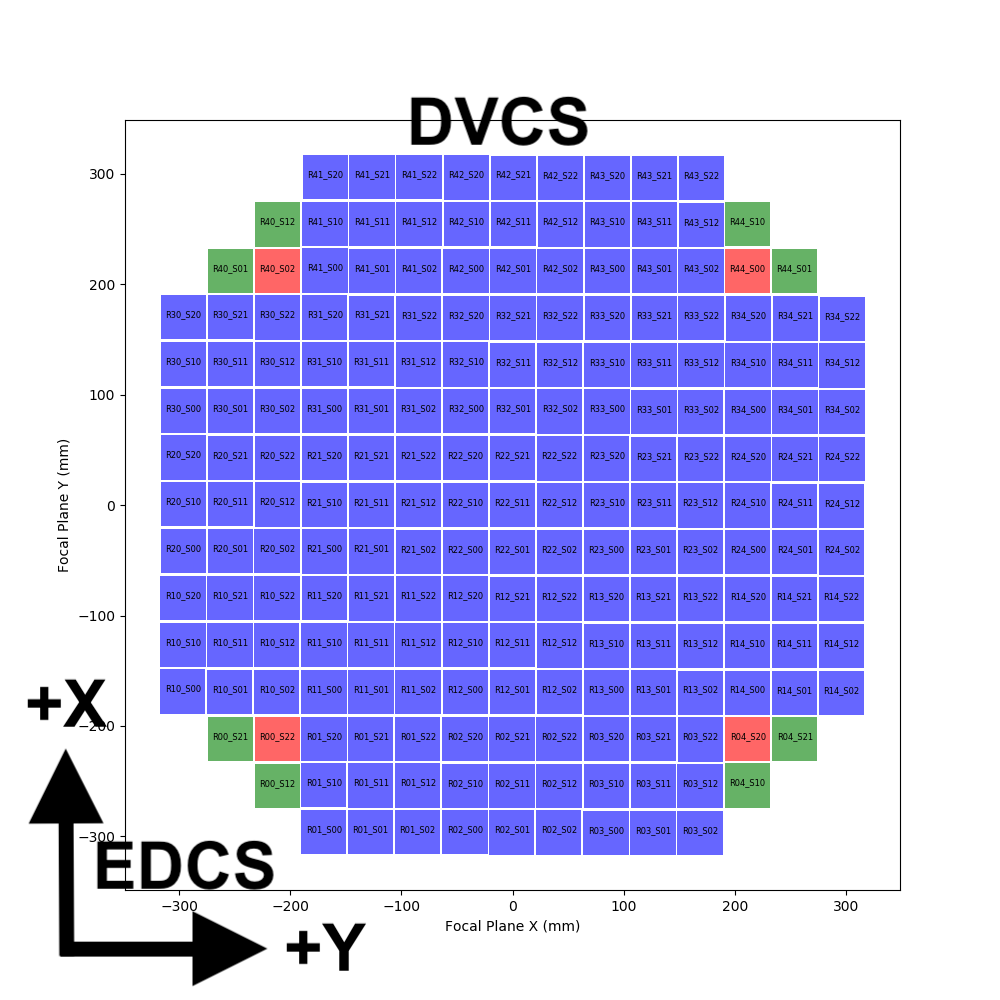
\includegraphics[width=0.75\textwidth]{figures/fp.png}
\captionof{figure}{This image is in the data visualization coordinate system (DVCS).  The engineering diagram coordinate system (EDCS) is shown in the lower left of the image.  Sensors are labeled following the convention in LCA-13381. Blue sensors are science sensors.  Red sensors are the wavefront sensors and green sensors are the guider chips.}
\end{center}
